%++++++++++++++++++++++++++++++++++++++++
% Don't modify this section unless you know what you're doing!
\documentclass[12pt,a4paper,tweside,onehalfspacing]{article}
\usepackage{natbib}
\bibliographystyle{unsrtnat}
\usepackage{tabularx} % extra features for tabular environment
\usepackage{amsmath}  % improve math presentation
\usepackage{graphicx} % takes care of graphic including machinery
\usepackage[margin=1in,letterpaper]{geometry} % decreases margins
%\usepackage{cite} % takes care of citations
\usepackage[final]{hyperref} % adds hyper links inside the generated pdf file
% Tabella usata nel frontespizio
\usepackage{tabularx}
% Per unire le celle delle tabelle
\usepackage{multirow}
% Per l'interlinea
\usepackage{setspace}
% Per rendere l'indice cliccabile
\usepackage{hyperref} 	
\hypersetup{
	colorlinks=true,       % false: boxed links; true: colored links
	linkcolor=blue,        % color of internal links
	citecolor=blue,        % color of links to bibliography
	filecolor=magenta,     % color of file links
	urlcolor=blue
}
\usepackage{bm}
\usepackage{circuitikz,siunitx}

%+++++++++++++++++++++++++++++++++++++++
\begin{document}

\thispagestyle{empty}

\begin{center}
	\begin{tabularx}{\textwidth}{cXc}
	\multirow{2}{2.7cm}{\centering \includegraphics[height=3cm]{"Frontespizio/logo-poli"}} & \centering {\bfseries \large Politecnico di Torino} & \multirow{2}{3.4cm}{\centering \includegraphics[height=3cm]{"Frontespizio/det"}} \\[5mm]
	& \centering {\scshape \large Department of Electronics and Telecommunications} & \\
	\end{tabularx} 
\end{center}

\vspace{5mm}

\begin{center}
	{\large PHYSICAL ENGINEERING}\\
	\vspace{\stretch{1}}
	{\Large Circuit Theory}\\

\end{center}

\vspace{\stretch{2}}


\begin{center}
	\begin{spacing}{2}
		{\bfseries \huge Switching behaviour of a Bistable circuit}
		
	\end{spacing}
\end{center}

\vspace{\stretch{2}}

\begin{center}
	\begin{tabularx}{\textwidth}{cXc}
	{\bfseries \large Professore:}	&&	{\bfseries \large Studente:}		\\
		&&		\\
	{\bfseries \large \itshape  Prof. Ivano Adolfo Maio}  &&	{\bfseries \large \itshape  Mattia Antonini mat.s281402}	\\
	&&		\\
    &&		\\	
    &&		\\

\end{tabularx}
\end{center}

%\bigskip

\hrule
\begin{center}
	{\bfseries\Large Academic Year 2021/22}
\end{center}
\newpage

\section{Introduction}

A \textbf{Bistable circuit} is an electronic circuit, usually an integrated circuit, whose output has two stable states to which it is directed by the input signal or signals. It is more usually known as a flip-flop. Binary states denote logic '1' and '0'.
A Bistable circuit is implemented as in  Fig. $\ref{bistable-circuit}$ and it is based on a negative-resistance converter.
%
\begin{figure}[!ht]
\begin{center}
\begin{circuitikz}[american, voltage shift=1]
\ctikzset{bipoles/length=1cm}
\draw (0, 0) node[op amp] (opamp) {}
(opamp.-) -- (-3, 0.35) to[short, -*] ++(0,-0.5) to[L=$L$, i<^=$i_L$, v=$v_L$] (-3,-1) to (-3,-1.1) to [V=$v_s(t)$, invert] (-3,-3) node[ground]{}
(opamp.down) node[ground] {}
(opamp.-) to[short,*-] ++(0,1) coordinate (leftC)
to[R=$R_f$] (leftC -| opamp.out)
to[short,-*] (opamp.out) to [short,-o] (1.5,0) node[above]{$v_o$} %to (1.5,-0.5) node[ground]{}
(opamp.+) -- (-0.85,-1.5) to[R=$R_2$] (-0.85,-2.5) -- (-0.85,-3) node[ground]{}
(-0.85,-1.2) to[R,l_=$R_1$] (0.85,-1.2) to[short,*-] (0.85,0)%(leftC -| opamp.out)
;
\end{circuitikz}
\caption{\small Bistable circuit based on OpAmp.} \label{bistable-circuit}
\end{center}
\end{figure}
%
\section{Negative-resistance converter}
A negative-resistance converter is shown here below in Fig. $\ref{Negative-resistance converter}$. Our task is to determine the driving-point characteristic of the Negative-resistance converter in the $i-v$ plane. We will analyze the behaviour of the Bistable circuit in the different regions of the driving-point characteristic.
%
\begin{figure}[!ht]
\begin{center}
\begin{circuitikz}[american, voltage shift=1]
\ctikzset{bipoles/length=1cm}
\draw (0,0) node[above]{} to[short, o-] ++(2,0)
node[op amp, anchor=-](OA){}
(OA.+) -- ++(0,-1) coordinate(FB)
to[R=$R_2$] ++(0,-2) node[ground]{$gnd$} coordinate (GND)
%(GND) to[short, o-] ++(-2,0) node[below]{$gnd$}
(0,-3.5) to[short, o-] ++(+2,0)
(0,0) to [open, v^>=$v$] (0,-4)
(OA.+) to [open, v^>=$v_d$] (OA.-)
(FB) to[R=$R_2$, *-] (FB -| OA.out) -- (OA.out)
to [short, *-o] ++(1,0) node[above]{$v_o$}
(OA.out) to[short,*-] ++(0,1.5) coordinate(NFB)
to[R=$R_f$,*-] (NFB -| OA.-)
to[short,-*] (OA.-)
;
\end{circuitikz}
\caption{\label{Negative-resistance converter}Negative-resistance converter.}
\end{center}
\end{figure}
We will replace the OpAmp of Fig. $\ref{Negative-resistance converter}$  by three circuit models for each of the regions where the Bistable circuit can work: the Linear region, the +Saturation region, the -Saturation region and for each of them the transient will be analyzed in depth.

\subsection{Linear region}
The OpAmp working in the Linear region can be modeled as in the next Fig. $\ref{linear-region}$.
%
\begin{figure}[!ht]
\begin{center}
\begin{circuitikz}[american, voltage shift=1]
\ctikzset{bipoles/length=1cm}
\draw (0,0) node[above]{v} to[short, o-] ++(2,0) coordinate (INPUTN)
(INPUTN) to[short,*-] ++(0,1.5) coordinate(FB)
(FB) to[R=$R_f$,*-] ++(2,0) to[short, o-] ++(0,-1)
to [cV=$Av_d$] ++(0,-3) to[short, o-] ++(0,-1) node[ground]{$gnd$}
(4,0.5) to[short, o-] ++(2,0) coordinate (OUTPUT)
to[short, o-] ++(1,0) node[above]{$v_o$}
(0,-5) to[short, o-] ++(2,0) coordinate (INPUTP)
(INPUTP) to[short, o-] ++(0,-0.2) node[ground]{$gnd$}
(INPUTP) to[short, o-] ++(0,1) to[R=$R_2$, *-] ++(0,1)
to[short, o-] ++(0,1) coordinate (FB)
to[short, o-] ++(1,0) to[R=$R_1$, *-] (FB -| OUTPUT) -- (OUTPUT)
(0,0) to [open, v^>=$v$] (0,-5)
(1,-2) to [open, v^>=$v_d$] ++(0,2)
(1,-2) to[short, o-] ++(1,0)
(1,-2) to [open, v^>=$v_2$] (1,-5)
(FB) to [R=$R_i$, *-] (INPUTN)
;
\end{circuitikz}
\caption{\label{linear-region}Negative-resistance converter: linear region.}
\end{center}
\end{figure}

\noindent By inspection of the equivalent circuit in Fig. \ref{linear-region} we note that $R_1$ and $R_2$ constitute a voltage divider so that
\begin{equation}\label{voltage_divider}
v_2=\frac{R_2}{R_1+R_2}v_0=\beta v_0
\end{equation}
In the linear region $v_d=0$ and so we can assume that $v=v_2$. Hence the previous equation ($\ref{voltage_divider}$) can be re-written as
%
\begin{subequations}
  \begin{equation}\label{voltage_divider_2}
    v=\beta v_o
\end{equation}
\begin{equation}\label{voltage_divider_3}
    v_o=\frac{v}{\beta}
\end{equation}
\end{subequations}
%
Applying KVL we obtain
\begin{equation}\label{linear_kvl}
    v=R_f i + v_o
\end{equation}
Substituting Equation (\ref{linear_kvl}) into Equation (\ref{voltage_divider_2}), we obtain
\begin{equation}\label{linear-iv-characteristic}
    i=-\left(\frac{R_1}{R_2}\right)\left(\frac{1}{R_f}\right)v
\end{equation}
%
To determine the boundary of these segments substitute equation(\ref{voltage_divider_2}) into the validating inequality
\begin{equation}
    -E_{sat} \leq v_o \leq E_{sat}
\end{equation}
Hence we get
\begin{equation}\label{linear_region_validity}
    -\beta E_{sat} \leq v \leq \beta E_{sat}
\end{equation}
%
Equation (\ref{linear_region_validity}) determines the range of validity for the input voltage $v$ in the Linear region.

\noindent It is important to remark that in this region the slope of the $i-v$ line is negative with value $-\frac{R_1}{R_2 R_f}$. Thus, we can claim that the resistance of the equivalent Norton circuit is
\begin{equation}
    \frac{v}{i}=-\frac{R_2 R_f}{R_1}
\end{equation}
The Bistable circuit in the Linear region can be modeled by the Norton equivalent circuit with a negative resistance, no source current, coupled to the inductor, show in Fig. $\ref{linear-norton-equivalent}$.
\begin{figure}[!ht]
\begin{center}
\begin{circuitikz}[american, voltage shift=2]
  \draw (0,0) to[R=-$R_{2} R_{f}/R_{1}$, i>_=$i_R$] (0,3);
  \draw (0,3) -- (2,3)
  to[L,l_=$L$, i>_=$i_L$, v^=$v_L$]
  (2,0) to[short, -*] (0,0);
\end{circuitikz}
\caption{\small Norton equivalent circuit for the OpAmp in the 'Linear' region.} \label{linear-norton-equivalent}
\end{center}
\end{figure}
\subsection{+ Saturation region}
When the OpAmp is operating on the '+ Saturation' the output voltage is $E_{sat}$. Hence the controlled voltage source of the 'Linear' region can be replaced by a battery with value $E_{sat}$.\\
\begin{figure}[!ht]
\begin{center}
\begin{circuitikz}[american, voltage shift=1]
\ctikzset{bipoles/length=1cm}
\draw (0,0) node[above]{v} to[short, o-] ++(2,0) coordinate (INPUTN)
(INPUTN) to[short,*-] ++(0,1.5) coordinate(FB)
(FB) to[R=$R_f$,*-] ++(2,0) to[short, o-] ++(0,-1)
to [battery=$E_{sat}$] ++(0,-3) to[short, o-] ++(0,-1) node[ground]{$gnd$}
(4,0.5) to[short, o-] ++(2,0) coordinate (OUTPUT)
to[short, o-] ++(1,0) node[above]{$v_o$}
(0,-5) to[short, o-] ++(2,0) coordinate (INPUTP)
(INPUTP) to[short, o-] ++(0,-0.2) node[ground]{$gnd$}
(INPUTP) to[short, o-] ++(0,1) to[R=$R_2$, *-] ++(0,1)
to[short, o-] ++(0,1) coordinate (FB)
to[short, o-] ++(1,0) to[R=$R_1$, *-] (FB -| OUTPUT) -- (OUTPUT)
(0,0) to [open, v^>=$v$] (0,-5)
(FB) to [open, v^>=$v_d$] ++(0,2)
(1,-2) to[short, o-] ++(1,0)
(1,-2) to [open, v^>=$v_2$] (1,-5)
;
\end{circuitikz}
\caption{\label{opamp-plus-saturation}Bistable circuit: + Saturation region.}
\end{center}
\end{figure}

\noindent By inspection of the equivalent circuit in  Fig. \ref{opamp-plus-saturation} and following the same procedure as above, we obtain
%
\begin{equation}
    v=R_f i+E_{sat}
\end{equation}
and so we get
%
\begin{subequations}\label{plus-saturation-characteristic}
  \begin{equation}
    i=\frac{v}{R_f}-\frac{E_{sat}}{R_f}
\end{equation}
\begin{equation}
    v_o=E_{sat}
\end{equation}
\end{subequations}
%
To determine the range of $v$ for which the previous two equations are valid, we solve for $v_d$ by applying KVL around the closed node sequence of the output stage of the OpAmp
\begin{equation}
    v_d=\frac{R_2}{R_1+R_2}E_{sat}-v=\beta E_{sat}-v
\end{equation}
The validating inequality for the '+ Saturation' region is
\begin{equation}
    v_d > 0
\end{equation}
Hence we obtain
\begin{equation}\label{plus-saturation-validity}
    v < \beta E_{sat}
\end{equation}
%
The Norton equivalent circuit for the '+ Saturation' region is shown here below in Fig. $\ref{plus-saturation-norton-equivalent}$.
\begin{figure}[!ht]
\begin{center}
\begin{circuitikz}[american, voltage shift=2]
  \draw (0,0) to[isource, l=$E_{sat}/R_f$] (0,3)
  to[short, -*, i=$i$] (2,3)
  to[R=$R_{f}$, i>_=$i_R$] (2,0) -- (0,0);
  \draw (2,3) -- (4,3)
  to[L,l_=$L$, i>_=$i_L$, v^=$v_L$]
  (4,0) to[short, -*] (2,0);
\end{circuitikz}
\caption{\small Norton equivalent circuit for the OpAmp in the '+ Saturation' region.} \label{plus-saturation-norton-equivalent}
\end{center}
\end{figure}
\subsection{- Saturation region}
The OpAmp working in the '- Saturation' region can be modeled as in Fig. $\ref{opamp-minus-saturation}$.
%
\begin{figure}[!ht]
\begin{center}
\begin{circuitikz}[american, voltage shift=1]
\ctikzset{bipoles/length=1cm}
\draw (0,0) node[above]{v} to[short, o-] ++(2,0) coordinate (INPUTN)
(INPUTN) to[short,*-] ++(0,1.5) coordinate(FB)
(FB) to[R=$R_f$,*-] ++(2,0) to[short, o-] ++(0,-1)
(4,0.5) to[battery, v<=$E_{sat}$, invert] ++(0,-3) to[short, o-] ++(0,-1) node[ground]{$gnd$}
(4,0.5) to[short, o-] ++(2,0) coordinate (OUTPUT)
to[short, o-] ++(1,0) node[above]{$v_o$}
(0,-5) to[short, o-] ++(2,0) coordinate (INPUTP)
(INPUTP) to[short, o-] ++(0,-0.2) node[ground]{$gnd$}
(INPUTP) to[short, o-] ++(0,1) to[R=$R_2$, *-] ++(0,1)
to[short, o-] ++(0,1) coordinate (FB)
to[short, o-] ++(1,0) to[R=$R_1$, *-] (FB -| OUTPUT) -- (OUTPUT)
(0,0) to [open, v^>=$v$] (0,-5)
(FB) to [open, v^>=$v_d$] ++(0,2)
(1,-2) to[short, o-] ++(1,0)
(1,-2) to [open, v^>=$v_2$] (1,-5)
;
\end{circuitikz}
\caption{\label{opamp-minus-saturation}Bistable circuit: - Saturation region.}
\end{center}
\end{figure}
%

\noindent By inspection of the circuit in Fig. \ref{opamp-minus-saturation} and following the same procedure as above we obtain
\begin{equation}
    v=R_f i-E_{sat}
\end{equation}
that leads to
\begin{subequations}
  \begin{equation}\label{minus-saturation-characteristic}
    i=\frac{v}{R_f}+\frac{E_{sat}}{R_f}
\end{equation}
%
\begin{equation}
    v_o=-E_{sat}
\end{equation}
\begin{equation}\label{minus-saturation-validity}
    v>-\beta E{sat}
\end{equation}
\end{subequations}
%
The Norton equivalent circuit is shown here below in Fig. $\ref{minus-saturation-norton-equivalent}$.
\begin{figure}[!ht]
\begin{center}
\begin{circuitikz}[american, voltage shift=2]
  \draw (0,0) to[isource, l=$-E_{sat}/R_f$] (0,3)
  to[short, -*, i=$i$] (2,3)
  to[R=$R_{f}$, i>_=$i_R$] (2,0) -- (0,0);
  \draw (2,3) -- (4,3)
  to[L,l_=$L$, i>_=$i_L$, v^=$v_L$]
  (4,0) to[short, -*] (2,0);
\end{circuitikz}
\caption{\small Norton equivalent circuit for the OpAmp in the '- Saturation' region.} \label{minus-saturation-norton-equivalent}
\end{center}
\end{figure}
%
\section{Circuit and driving-point characteristic}
As we have explained previously, a Bistable circuit can be implemented by the circuit shown in Fig. $\ref{bistable-circuit}$.
Further the driving-point characteristic obtained in the previous paragraphs is shown here below.
\begin{figure}[!ht]
        \centering 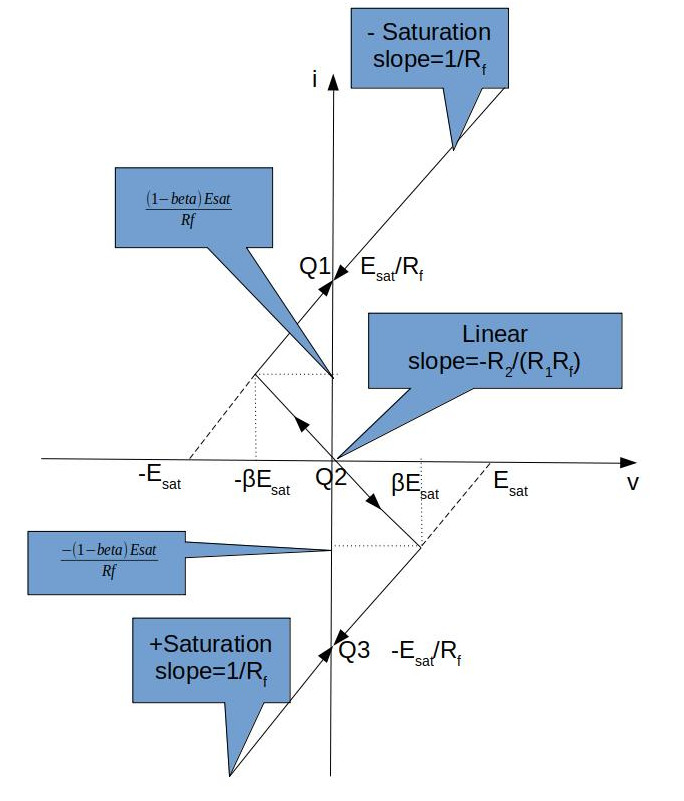
\includegraphics[width=0.8\columnwidth]{driving-point-characteristic.jpg}\caption{\label{driving-point characteristic}Bistable circuit: driving-point characteristic.
        }
\end{figure}
Consider first the case where $v_s(t) = 0$ so that the inductor is directly connected across the circuit. Since $\frac{di(t)}{dt}=-v(t)/L$ and $L>0$, it follows that $\frac{di(t)}{dt}>0$ whenever $v < 0$ and $\frac{di(t)}{dt} < 0$ whenever $v>0$.\\
Hence, the current $i$ decreases in the right half $v-i$ plane and increases in the left half $v-i$ plane, as depicted by the typical dynamic routes in Fig. \ref{driving-point characteristic}.\\
Since the equilibrium state of a first order RL circuit is determined by replacing the inductor by a short circuit, i.e. $v=v_L=0$, it follows that this circuit has three equilibrium points: $Q_1$, $Q_2$ and $Q_3$. These equilibrium points are the operating points of the associated resistive circuit obtained by short-circuiting the inductor $L$.\\
Since the dynamic route in Fig. \ref{driving-point characteristic} either tends to $Q_1$ or $Q_3$, but always diverges from $Q_2$, we say that the equilibrium point $Q_2$ is unstable. Hence even though the associated resistive circuit has three operating points, $Q_2$ can never be observed in practice (the slightest noise voltage will cause the dynamic route to diverge from $Q_2$, even if the circuit is operating initially at $Q_2$.\\
Whether $Q_1$ or $Q_3$ is actually observed depends on the initial condition. Such a circuit is said to be bistable.\\
Bistable circuits (flip-flops) are used extensively in digital computers, where the two stable equilibrium points correspond to the two binary states; say $Q_1$ denotes $'0'$ and $Q_3$ denotes $'1'$.\\
In order to perform logical operations, it is essential to switch from $Q_1$ to $Q_3$ and vice versa. This is done by using a small triggering signal. We will now show how the voltage source in Fig. \ref{bistable-circuit} serves as a triggering signal.

\section{Some helpful equations}
As we have shown previously the Bistable circuit can be modeled as three RL circuits for each of the regions where it can work (Linear, +Saturation, -Saturation).
In the following analysis it will be helpful to evaluate at what time $t_k$ the current $i(t)$ through the inductor gets a specific value $i(t_k)$ knowing the initial time $t_j$, the current value $i(t_{\infty})$ for $t\rightarrow+\infty$ (or for $t\rightarrow-\infty$). Hence the following formula will be used along the way.
\begin{equation}\label{time-evaluation}
    t_k - t_j=\tau log \left(\frac{i(t_j)-i(t_{\infty})}{i(t_k)-i(t_{\infty})}\right)
\end{equation}
This formula doesn't depend on whether $\tau$ is positive or negative. It will be used also for the linear region where the $G_{eq}$ is negative ($-\frac{R_1}{R_2 R_f}$).\\
It will be useful also to compute the value of the current $i(t)$ at a specific time knowing the initial current value $i(t_0)$ and the current value $i(t_{\infty})$ for $t\rightarrow+\infty$ (or for $t\rightarrow-\infty$).
\begin{equation}
    i(t)=i(t_{\infty}) + [i(t_0)-i(t_{\infty})]e^{\frac{-(t-t_0)}{\tau}}
\end{equation}
which holds for all times $t$, i.e. $-\infty < t < +\infty$ and for $\tau$ positive or negative (in the Linear region).
Depending on whether $\tau$ is positive or negative, the exponential waveform tends either to a constant or to $\infty$ as the time $t$ tends to $\infty$.
The switching analysis will start from a known stable point ($Q_1$ for instance) and then applying a voltage impulse to the inductor voltage in order to force a transient. Then the inductor current will move along the piecewise characteristic in the $i-v$ plane.
%
\section{Switching analysis}
Assume that the circuit first is working in $Q_1$. We know that this is a stable equilibrium point. A constant (negative) current $i_L$ is flowing through the inductor $L$. The voltage across the inductor $L$ is $0$. The OpAmp is working in saturation (-Saturation region) and, thus, its output voltage is $v_o=-E_{sat}$.
%
\begin{subequations}
  \begin{equation}
v_o=-E_{sat}
\end{equation}
\begin{equation}
v=0
\end{equation}
\begin{equation}
v_d=v_2-0=\frac{R_2}{R_1+R_2}v_o=-\frac{R_2}{R_1+R_2}E_{sat}<0
\end{equation}
\begin{equation}
i=\frac{v-v_o}{R_f}=\frac{0-(-E_{sat})}{R_f}=\frac{E_{sat}}{R_f}
\end{equation}
The derivative of the current $\frac{di_L(t)}{dt}$ is '0'. The circuit will not move from this point unless a triggering signal will be applied by the voltage source $v_s(t)$ (see Fig. \ref{bistable-circuit}).\\
Let us at $t=t_1$ apply a square pulse of width $T=t_2-t_1$ and amplitude $E$ (see Fig. $\ref{positive-pulse}$).
\begin{equation}
    E_s(t)=E(u(t_1)-u(t_2))
\end{equation}
\end{subequations}
%
\begin{figure}[!ht]
        \centering 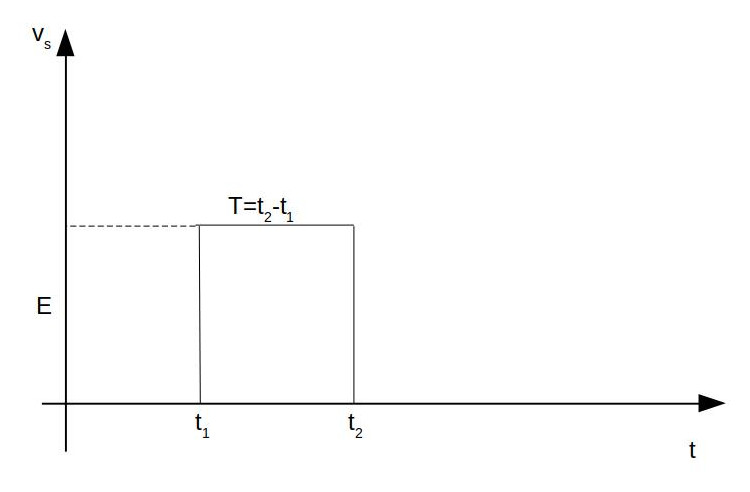
\includegraphics[width=0.9\columnwidth]{positive-pulse}
        \caption{\label{positive-pulse} Triggering positive pulse.
        }
\end{figure}
During the  time interval $t_1 \leq t \leq t_2$, $v_s(t)$ can be replaced by a battery $E$ so that the inductor sees a translated driving-point characteristic as shown in Fig. \ref{set-signal-translated-driving-point} (see dashed line).
%
\begin{figure}[!ht]
        \centering 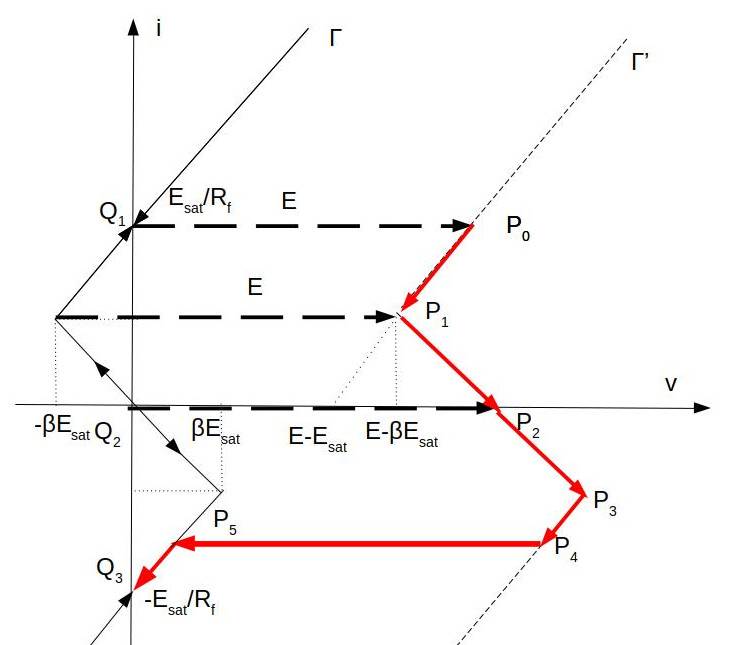
\includegraphics[width=0.9\columnwidth]{driving-point-characteristic-shifted.jpg}
        \caption{\label{set-signal-translated-driving-point}Translated 'driving-point' characteristic.
        }
\end{figure}
Now the voltage across the inductor is greater than '0'. In other words the two pins across the inductor are at different voltages, the upper is still at $0$ Volts, while the lower is at $-E$ Volts. The voltage across the inductor is
\begin{equation}
    v_L=v=E
\end{equation}
Let us denote the original and the translated piece wise-linear driving-point characteristics by $\Gamma$ and $\Gamma^{'}$ respectively. See Fig. $\ref{set-signal-translated-driving-point}$. The $\Gamma$ holds over the time interval $t \leq t_1$ and $t\geq t_2$, whereas $\Gamma^{'}$ holds over the time interval $t_1 \leq t \leq t_2$.
Since the inductor current cannot change instantaneously $i_L(t_1^{-})=i_L(t_1^{+})$, the dynamic route must jump horizontally from $Q_1$ to $P_0$ at time $t=t1$. The $\Gamma$ driving-point characteristic has been horizontally translated of $E$ Volts to the right.
The circuit can be modeled taking its Norton equivalent circuit as shown in Fig. $\ref{minus-saturation-norton-equivalent-shifted}$. The conductance is the slope of the driving-point characteristic (see Fig. $\ref{driving-point characteristic}$).
\begin{figure}[!ht]
\begin{center}
\begin{circuitikz}[american, voltage shift=2]
  \draw (0,0) to[isource, l=($E-E_{sat})/R_f$] (0,3)
  to[short, -*, i=$i$] (2,3)
  to[R=$1/R_{f}$, i>_=$i_R$] (2,0) -- (0,0);
  \draw (2,3) -- (4,3)
  to[L,l_=$L$, i>_=$i_L$, v^=$v_L$]
  (4,0) to[short, -*] (2,0);
\end{circuitikz}
\caption{\small Norton equivalent circuit for the OpAmp in the shifted '- Saturation' region.} \label{minus-saturation-norton-equivalent-shifted}
\end{center}
\end{figure}
From $P_0$ the current $i$ must subsequently decrease so long as $v \geq 0$ towards $P_1$ with slope $\frac{1}{R_f}$. In that region the Bistable circuit is in the '- Saturation' region as indicated in Fig. $\ref{set-signal-translated-driving-point}$ and so it will modeled as a $RL$ circuit described in Fig. $\ref{minus-saturation-norton-equivalent}$ and ruled by the equations (\ref{minus-saturation-characteristic}). Hence, the input current $i(t)$ to the Bistable circuit will evolve as a decreasing exponential with time constant $\tau=\frac{L}{R}$.
\begin{equation}
    i(t)=\frac{E-E_{sat}}{R_f}+[i(P_0) -\frac{E-E_{sat}]}{R_f}e^{\frac{-t}{\tau}}
\end{equation}
We can claim that
%
\begin{subequations}
  \begin{equation}
    i_{P_0}(E)=i(Q_1)=\frac{E_{sat}}{R_f}
\end{equation}
\begin{equation}
    i_{P_1}(E-\beta E_{sat})=\frac{E_{sat}(1-\beta)}{R_f}
\end{equation}
\begin{equation}
    i(t_{\infty})=\frac{E-E_{sat}}{R_f}
\end{equation}
By the equation($\ref{time-evaluation}$) after some manipulation we obtain:
\begin{equation}
    t_{P_1}=t_{P_0} +\tau \log\left(\frac{2E_{sat}-E}{E_{sat}(2+\beta)-E}\right)
\end{equation}
\end{subequations}
%
The transient in the '- Saturation' region evolves from $P_0$ to $P_1$, but there the behaviour will be driven by the 'Linear' region (negative slope $-\frac{R_1}{R_2 R_f}$) where the Bistable circuit is ruled by the following equations and values:
\begin{equation}
    i(t)=-\frac{R_1(v-E)}{R_2 R_f}
\end{equation}
From the analysis in the '- saturation' region we know that
%
\begin{subequations}
  \begin{equation}
    i(P_1)=\frac{E_{sat}(1-\beta)}{R_f}
\end{equation}
\begin{equation}
    v(P_1)= E+\beta E_{sat}
\end{equation}
\begin{equation}
    i(P_3)=-i(P_1)=-\frac{E_{sat}(1-\beta)}{R_f}
\end{equation}
\end{subequations}
%
In the 'Linear' region the time constant of the circuit has a negative value and can be expressed as
\begin{equation}
    \tau_{lin}=\frac{L}{R_{eq}}=-\frac{R_1 L}{R_2 R_f}
\end{equation}
%
In the 'Linear' region the Bistable circuit is modeled by the following Norton equivalent circuit (see Fig. $\ref{linear-norton-equivalent-shifted}$).
%
\begin{figure}[!ht]
\begin{center}
\begin{circuitikz}[american, voltage shift=2]
  \draw (0,0) to[isource, l=-($E)\frac{R_1}{R_2 R_f}$] (0,3)
  to[short, -*, i=$i$] (2,3)
  to[R=-$\frac{R_1}{R_2 R_f}$, i>_=$i_R$] (2,0) -- (0,0);
  \draw (2,3) -- (4,3)
  to[L,l_=$L$, i>_=$i_L$, v^=$v_L$]
  (4,0) to[short, -*] (2,0);
\end{circuitikz}
\caption{\small Norton equivalent circuit for the OpAmp in the shifted 'Linear' region.} \label{linear-norton-equivalent-shifted}
\end{center}
\end{figure}
%

\noindent Because of the negative time constant $\tau$ the $RL$ circuit is unstable and exponentially growing when $t$ tends to $\infty$. The $i(t)$ function is stable when $t$ tends to $-\infty$. The current value tends to current generator $i_{eq}$ value $-E\frac{R1}{R_2 R_f}$ when $t\rightarrow\-\infty$. In the 'Linear' region the current $i(t)$ evolves according to the following exponential expression valid for $t_{P_1} < t < t_{P_3}$:
%
\begin{subequations}
  \begin{equation}
    i(t)=(i(P_1) - i_{eq})e^{-\frac{t-t(P_1)}{\tau_{lin}}}
\end{equation}
\begin{equation}
    t_{P_3}=t_{P_1} + \tau_{lin}log(\frac{i(P_1) - i(t_{-\infty})}{i_{P_3}-i(t_{-\infty})})
\end{equation}
\begin{equation}
    v(P_3)= E + E_{sat}
\end{equation}
\end{subequations}
%
In the point $P_3$ the behaviour of the circuit changes once more. From $P_3$ to $P_4$ the circuit works in the '+ Saturation' state. It can be modeled by the following Norton equivalent circuit shown in Fig. $\ref{plus-saturation-norton-equivalent-shifted}$.
\begin{figure}[!ht]
\begin{center}
\begin{circuitikz}[american, voltage shift=2]
  \draw (0,0) to[isource, l=($E+E_{sat})/R_f$] (0,3)
  to[short, -*, i=$i$] (2,3)
  to[R=$1/R_{f}$, i>_=$i_R$] (2,0) -- (0,0);
  \draw (2,3) -- (4,3)
  to[L,l_=$L$, i>_=$i_L$, v^=$v_L$]
  (4,0) to[short, -*] (2,0);
\end{circuitikz}
\caption{\small Norton equivalent circuit for the OpAmp in the shifted '+ Saturation' region.} \label{plus-saturation-norton-equivalent-shifted}
\end{center}
\end{figure}

\noindent The time constant is positive with value $\tau=\frac{L}{R_f}$.
The time evaluation of the current $i(t)$ is ruled by the following expression from $P_3$ and beyond:
\begin{equation}
    i(t)=\left(i(P_3) -\frac{E+E_{sat}}{R_f}\right)e^{-\frac{t-t(P_3)}{\tau}}+\frac{E+E_{sat}}{R_f}
\end{equation}
This is a stable exponentially growing evolution that tends to the value $\frac{E+E_{sat}}{R_f}$ for $t\rightarrow\infty$.\\
Assume now that the $t_2$ occurs during this phase and so the voltage source $v_s(t)$ goes to $0$. At time $t=t_2$ the driving-point characteristic $\Gamma'$ switches back to $\Gamma$ and the dynamic route must jump horizontally from $P_4$ to $P_5$ at $t=t_2^{+}$. Then, from $P_5$ to $Q_3$ the dynamic route will move along the initial driving-point characteristic until it reaches the stable point $Q_3$. In $Q_3$ the voltage $v=0$ and also the derivative of the current through the inductor $\frac{di_L}{dt}$. Hence, the Bistable circuit will not move out from $Q_3$. It has been forced to change its steady state.\\
%
To trigger from $Q_3$, back to $Q_1$, simply apply a similar triggering pulse of opposite polarity, as shown in Fig.($\ref{triggering-reset-signal-translated-driving-point2}$). The resulting dynamic route is shown in Fig. \ref{triggering-reset-signal-translated-driving-point2}.
%
\begin{figure}[!ht]
        \centering 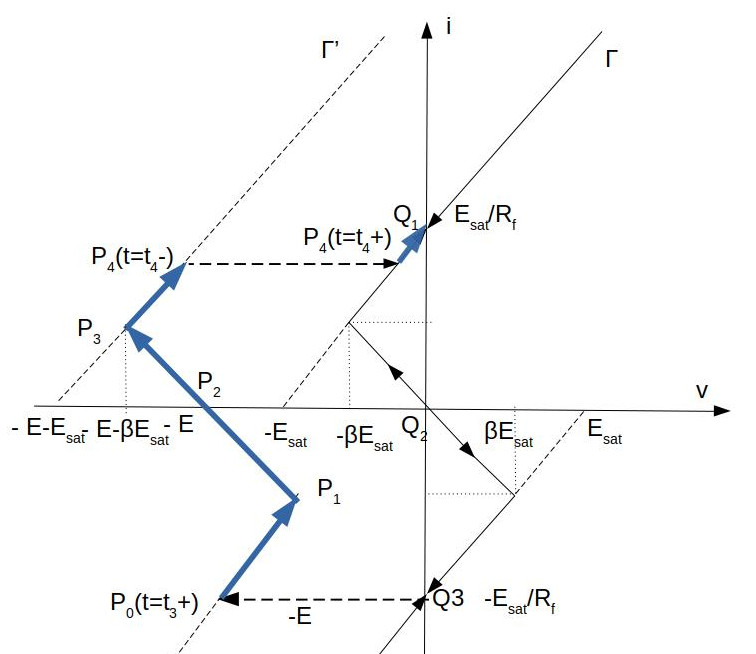
\includegraphics[width=0.9\columnwidth]{driving-point-characteristic-back-shifted.jpg}
        \caption{\label{triggering-reset-signal-translated-driving-point2}Triggering reset signal and translated 'driving-point' characteristic.
        }
\end{figure}
%
The Bistable circuit behaviour from $Q_3$ to $Q_1$ will be based on the same concepts described in the previous section, only the direction of the dynamic route will be the opposite.
%
\section{LTspice simulations}
\subsection{Schematic}
The schematic entry used in LTspice to simulate the Bistable behaviour is show in Fig. $\ref{LTspice_schematic}$
\begin{figure}[!ht]
        \centering 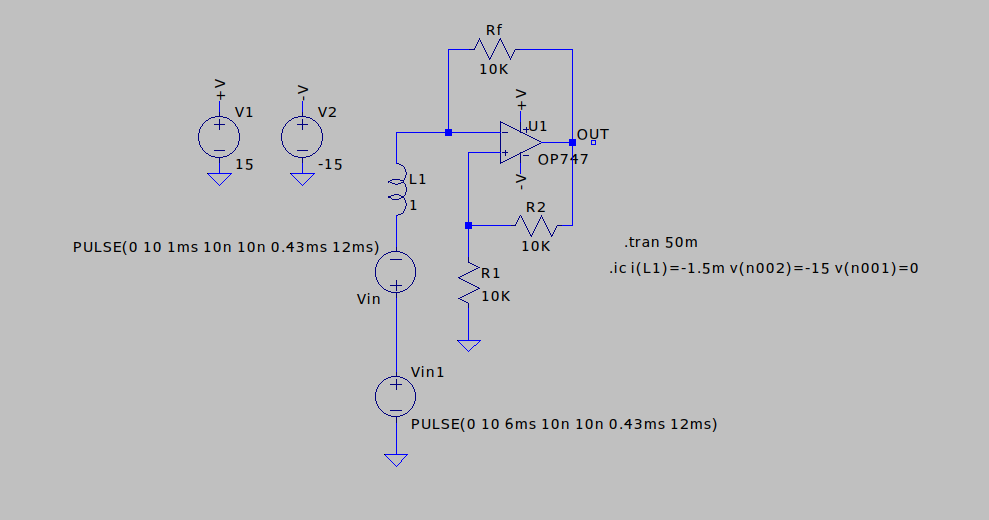
\includegraphics[width=0.8\columnwidth]{bistable-schematic.png}
        \caption{\label{LTspice_schematic}LTspice schematic used for simulation.
        }
\end{figure}
%
\subsection{Initial Conditions}
In order to force the circuit to start from the stable point $Q_1$ specific initial conditions were required for the inductor current $i_L=-\frac{E_{sat}}{R_f}$, the input voltage ($v=0$) and output voltage $v_o=-E_{sat}$. The initial conditions have been specified by the $.ic$ directive (see the appendix for all the netlist details).
\begin{verbatim}
.ic i(L1)=-1.5m v(n002)=-15 v(n001)=0
\end{verbatim}
%
\subsection{First simulation: pulse width \texorpdfstring{$\bm{T=0.415\ ms}$}{} }
In the first simulation the pulse width has been set to a specific value in order to reproduce the behaviour shown in  Fig. $\ref{set-signal-translated-driving-point}$. In other words when the pulse goes to $0V$ the dynamic route jumps back and the point $P_5$ is still in the right side of the $i-v$ plane. Thus, the following transient from $P_5$ to $Q_3$ occurs as a growing exponential for $i_L$ or a decreasing exponential for $i$.
The SPICE syntax for a voltage source is
\begin{verbatim}
Vin1 N005 0 PULSE(0 10 6ms 10n 10n 0.415ms 12ms)
\end{verbatim}
%
\begin{figure}[!ht]
        \centering 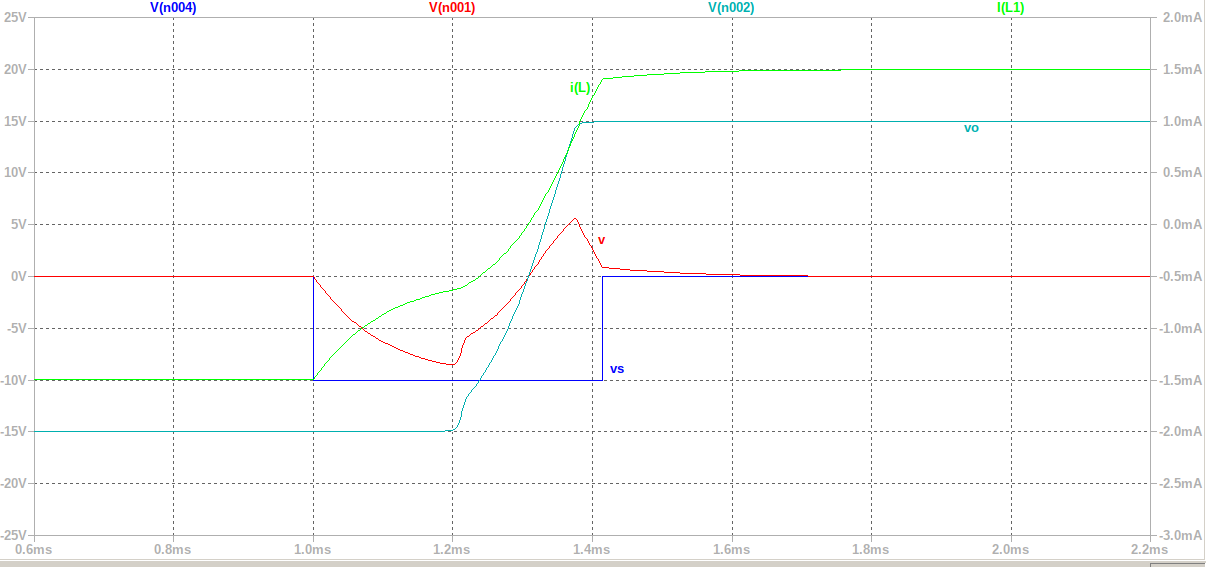
\includegraphics[width=0.8\columnwidth]{first-simulation-Q1-Q3.png}
        \caption{\label{first-simulation-q1-q3}First simulation: $T=0.415\ ms$, from $Q_1$ to $Q_3$.
        }
\end{figure}
%
As expected the inductor current $i_L$ grows as an exponential with positive time constant in the phase ('- Saturation' region). In the 'Linear region' the current grows with a negative time constant. It would tends to $+\infty$ (unstable behaviour) but when the dynamic route enters the '+ Saturation' region the behaviour returns to be stable. It will grow exponentially, but it would tend to a finite value for $t\rightarrow+\infty$.\\
The output voltage (red line) jumps from $-E_{sat}$ (logical '0') to $E_{sat}$ (logical '1').\\
The transition from $Q_3$ to $Q_1$ can be triggered by an opposite signal to the voltage source $v_s$ as depicted in Fig. $\ref{first-simulation-q3-q1}$.
%
\begin{figure}[!ht]
        \centering 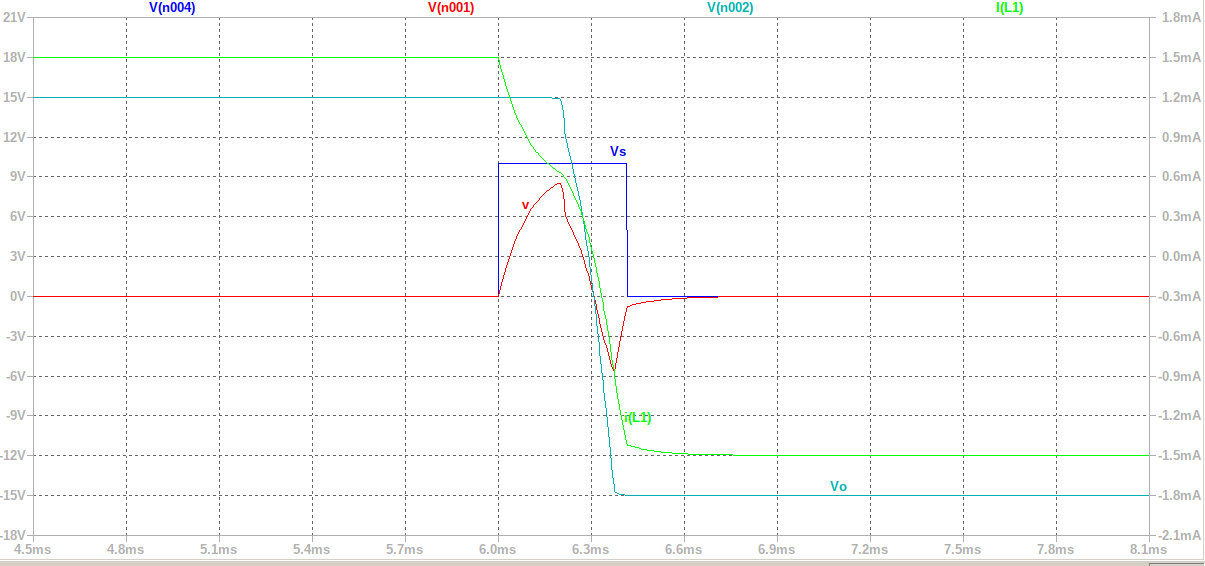
\includegraphics[width=0.8\columnwidth]{first-simulation-Q3-Q1.png}
        \caption{\label{first-simulation-q3-q1}First simulation: T=0.415ms, from $Q_3$ to $Q_1$.
        }
\end{figure}
%
\clearpage
%
\newpage
%
\subsection{Second simulation, pulse width \texorpdfstring{$T=0.45\ ms$}{}}
In this second simulation we are going to increase the pulse width so that when the voltage source returns to $0$ the dynamic route will jump in the left side of the $i-v$ plane and so the transient from $P_5$ to $Q_3$ will be different from the previous one.
%
\begin{verbatim}
    Vin1 N005 0 PULSE(0 10 6ms 10n 10n 0.45ms 12ms)
\end{verbatim}
\begin{figure}[!ht]
        \centering 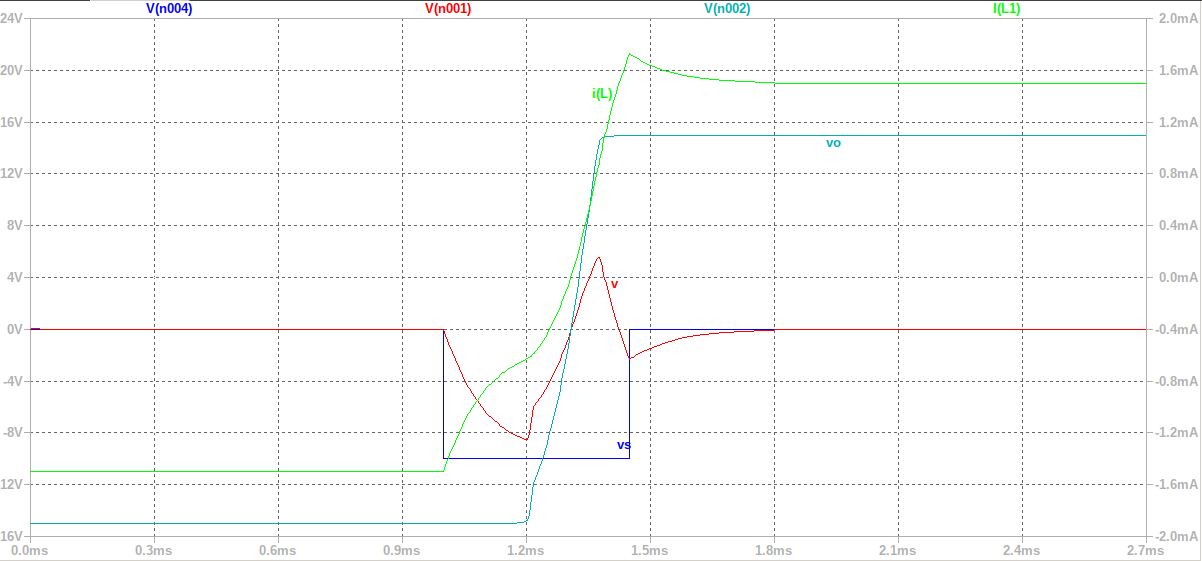
\includegraphics[width=0.8\columnwidth]{second-simulation-Q1-Q3.png}
        \caption{\label{second-simulation-q1-q3}Second simulation: $T=0.45\ ms$, from $Q_1$ to $Q_3$.
        }
\end{figure}
The different behaviour is evident at the end of the triggering pulse because the inductor current $i_L$ has grown over the steady value and so it decreases a bit to reach the steady state.\\
In other words when the triggering pulse goes to $0$ the point $P5$ will be in the left side of the $i-v$ plane. The output voltage (red line) will be forced to jump from the logical value $0$ ($Q_1$) to the logical value $0$ ($Q_3$). Fig. $\ref{second-simulation-q3-q1}$ shows the opposite transition from $Q_3$ to $Q_1$. The transient is the dual of the previous one.
\begin{figure}[!ht]
        \centering 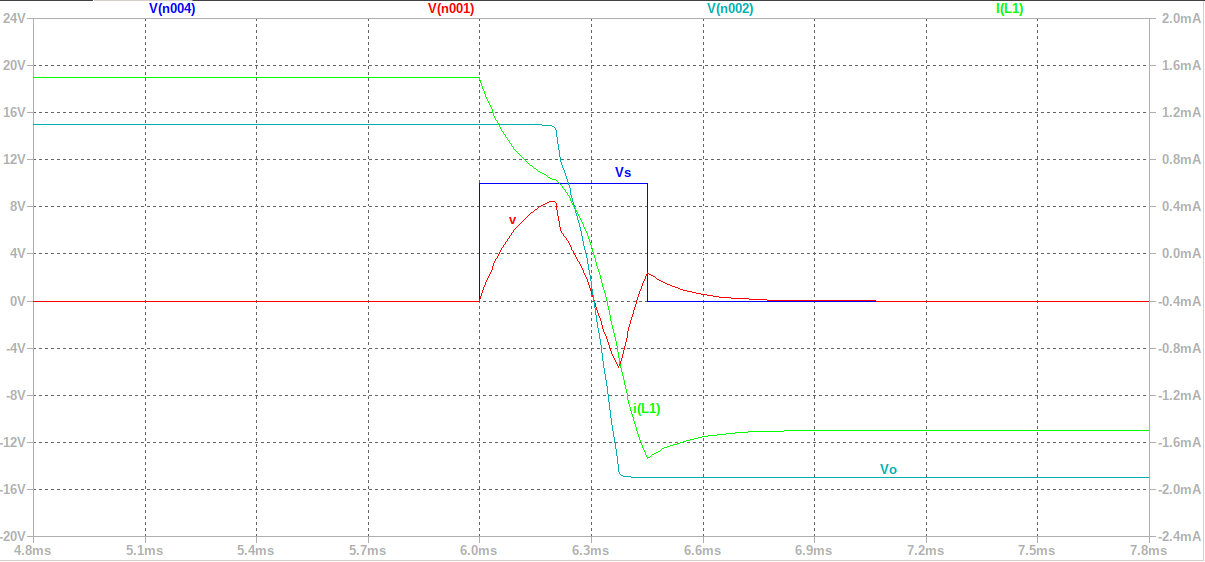
\includegraphics[width=0.8\columnwidth]{second-simulation-Q3-Q1.png}
        \caption{\label{second-simulation-q3-q1}Second simulation: $T=0.45\ ms$, from $Q_3$ to $Q_1$.
        }
\end{figure}
%
\clearpage
%
\newpage
%
\subsection{Third simulation, pulse width \texorpdfstring{$T$}{} too short, no transition}
When the triggering pulse is too short the transition will not occur. The third simulation shows this (bad) behaviour. The triggering pulse width is just $0.1\ ms$. Hence when the triggering pulse return to $0$ the dynamic route is still in the '- Saturation' region and so the dynamic route will jump back to the left side of the $i-v$ plane. The dynamic point will return back to $Q_1$ by a decreasing exponential. No transition takes place and the output voltage (red line) will remain at the logical value $0$.
In this case the dynamic route will move as in Fig. $\ref{dynamic-route-short-width}$.
\begin{figure}[!ht]
        \centering 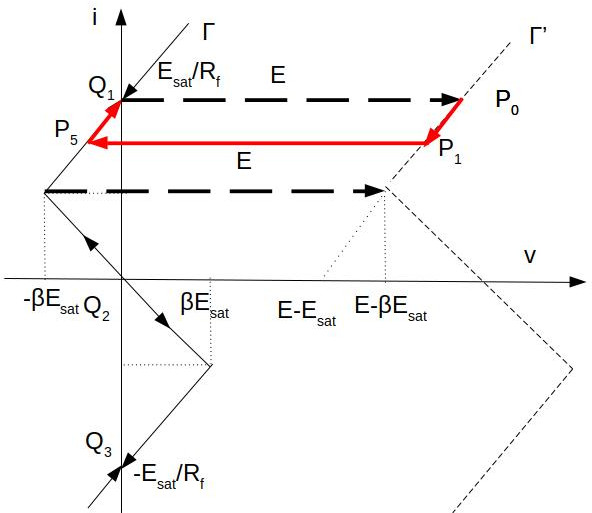
\includegraphics[width=0.6\columnwidth]{driving-point-characteristic-short-width-shifted.jpg}
        \caption{\label{dynamic-route-short-width} Third simulation: dynamic route, no transition.
        }
\end{figure}


\noindent The inductor transient current and voltages are depicted in Fig. $\ref{third-simulation-short-width}$.
%
\begin{figure}[!ht]
        \centering 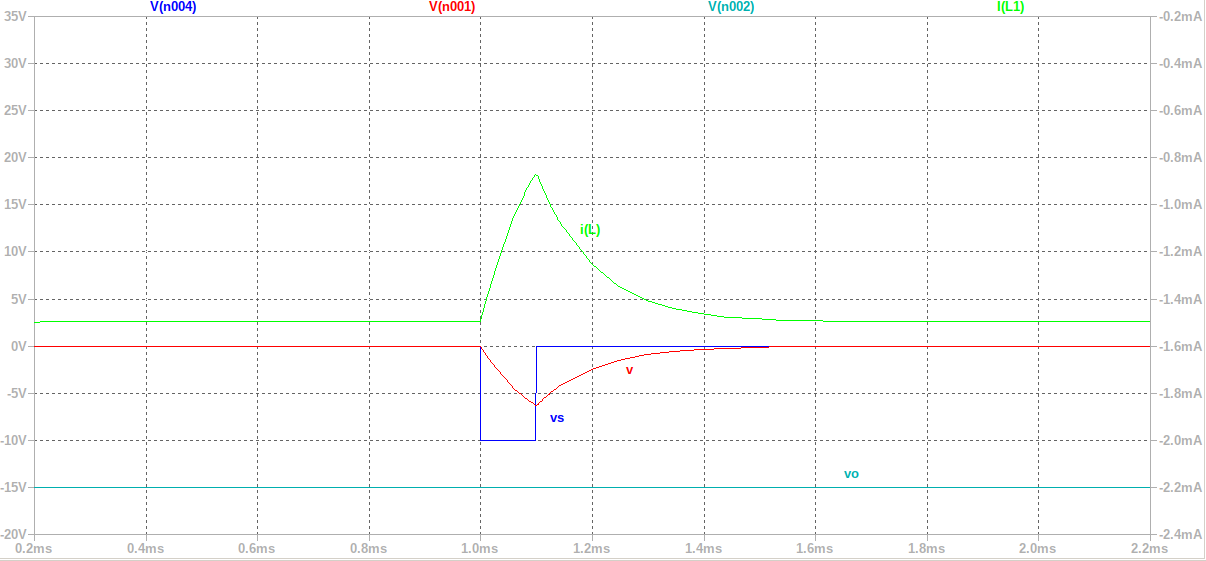
\includegraphics[width=0.8\columnwidth]{width-short-no-transition.png}
        \caption{\label{third-simulation-short-width}Third simulation: width too short $T=0.1\ ms$, no transition.
        }
\end{figure}
%
\clearpage
%
\newpage
%
\subsection{Fourth simulation, pulse width \texorpdfstring{$T=0.415\ ms$}{}, but pulse amplitude to small (2\ V), no transition}
The transition will not occur whenever the pulse amplitude is too small. In the fourth simulation the amplitude has been set to $2\ V$.
%
\begin{figure}[!ht]
        \centering 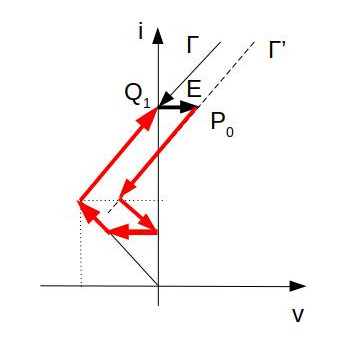
\includegraphics[width=0.6\columnwidth]{driving-point-characteristic-low-amplitude-shifted.jpg}
        \caption{\label{fourth-simulation-driving-point}Fourth simulation: amplitude too short, no transition.
        }
\end{figure}

\noindent In this case, the breakpoint $P_1$ on $\Gamma'$ is located in the left side of the plane. During this transient, the dynamic route will intercept the vertical axis and so the transient will stop in this point until the end of the triggering pulse. Then it will return to $\Gamma$ back to $Q_1$ and no logical transition will occur. In order to have a transition the pulse amplitude must be:
\begin{equation}
    E > \beta E_{sat}
\end{equation}
or
\begin{equation}
    E < -\beta E_{sat}
\end{equation}
\begin{figure}[!ht]
        \centering 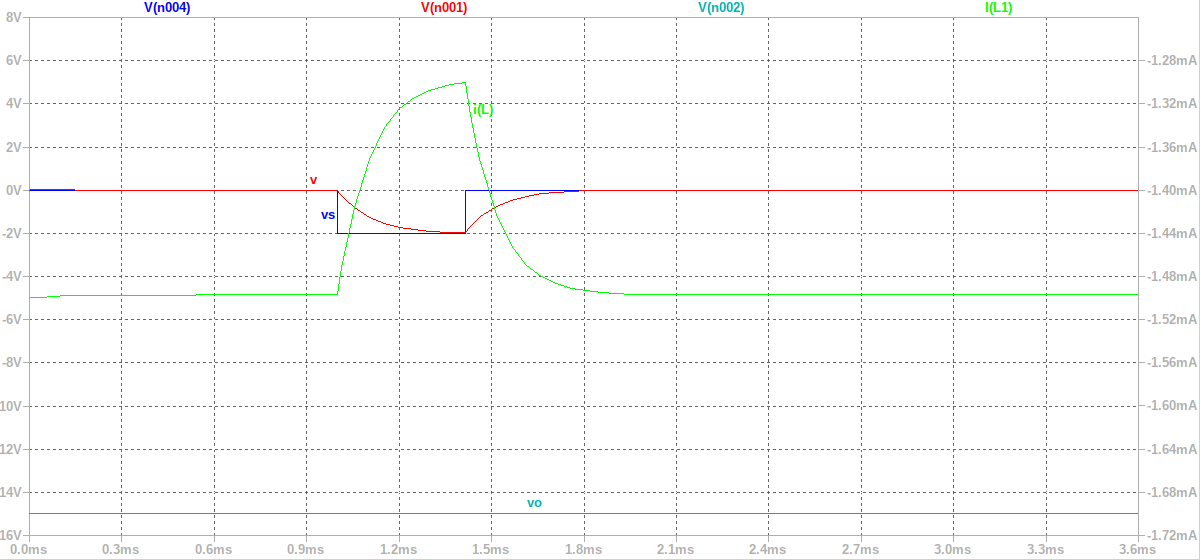
\includegraphics[width=0.8\columnwidth]{amplitude-short-no-transition.png}
        \caption{\label{fourth-simulation-amplitude-short}Fourth simulation: amplitude too short $(2\ V), T=0.415\ ms$, no transition.
        }
\end{figure}
%
%\clearpage
%\newpage
%
\section{Conclusion}
%
In the present short paper the switching behavior of a Bistable circuit has been analyzed. The Bistable circuit has been modeled by three different RL equivalent circuits. In other words, the Bistable circuit has been described by a piecewise-linear driving-point characteristic.\\
Finally, some LTspice simulations have been run to dive into the transient behaviour of the circuit changing the triggering pulse width and amplitude. The SPICE netlist has been provided.
%
\begin{thebibliography}{99}
\bibitem[\protect\citeauthoryear{}{2010}]{Author2010}
%\bibitem{Author2010}
Leon O. Chua, Charles A. Desoer, Ernest S. Kuh, - Linear and Nonlinear Circuits (1987), McGraw-Hill College.
\bibitem[\protect\citeauthoryear{}{2021}]{Author2021}
%\bibitem{Author2021}
Simon Bramble, - LTspice Tutorial.
\end{thebibliography}

%\begin{thebibliography}{9}
%\bibitem{Chua87DK}
%Leon O. Chua, Charles A. Desoer, Ernest S. Kuh (1987) \emph{Linear and Nonlinear Circuits}, McGraw-Hill College.
%
%\bibitem{LTspice}
%Simon Bramble, \emph{LTspice Tutorial}.
%\end{thebibliography}
%
\clearpage
%
\appendix
%
\section{LTspice netlist: bistable circuit}
V1 +V 0 15\\
Vin N005 N004 PULSE(0 10 1ms 10n 10n 0.415ms 12ms)\\
R1 N003 0 10K\\
R2 N002 N003 10K\\
XU1 N003 N001 +V -V N002 OP747\\
V2 -V 0 -15\\
L1 N001 N004 1\\
Rf N002 N001 10K\\
Vin1 N005 0 PULSE(0 10 6ms 10n 10n 0.415ms 12ms)\\
.tran 50m\\
.ic i(L1)=-1.5m v(n002)=-15 v(n001)=0\\
.lib ADI.lib\\
.backanno\\
.end\\
\end{document}
